% Options for packages loaded elsewhere
% Options for packages loaded elsewhere
\PassOptionsToPackage{unicode}{hyperref}
\PassOptionsToPackage{hyphens}{url}
\PassOptionsToPackage{dvipsnames,svgnames,x11names}{xcolor}
%
\documentclass[
  letterpaper,
  DIV=11,
  numbers=noendperiod]{scrartcl}
\usepackage{xcolor}
\usepackage{amsmath,amssymb}
\setcounter{secnumdepth}{-\maxdimen} % remove section numbering
\usepackage{iftex}
\ifPDFTeX
  \usepackage[T1]{fontenc}
  \usepackage[utf8]{inputenc}
  \usepackage{textcomp} % provide euro and other symbols
\else % if luatex or xetex
  \usepackage{unicode-math} % this also loads fontspec
  \defaultfontfeatures{Scale=MatchLowercase}
  \defaultfontfeatures[\rmfamily]{Ligatures=TeX,Scale=1}
\fi
\usepackage{lmodern}
\ifPDFTeX\else
  % xetex/luatex font selection
\fi
% Use upquote if available, for straight quotes in verbatim environments
\IfFileExists{upquote.sty}{\usepackage{upquote}}{}
\IfFileExists{microtype.sty}{% use microtype if available
  \usepackage[]{microtype}
  \UseMicrotypeSet[protrusion]{basicmath} % disable protrusion for tt fonts
}{}
\makeatletter
\@ifundefined{KOMAClassName}{% if non-KOMA class
  \IfFileExists{parskip.sty}{%
    \usepackage{parskip}
  }{% else
    \setlength{\parindent}{0pt}
    \setlength{\parskip}{6pt plus 2pt minus 1pt}}
}{% if KOMA class
  \KOMAoptions{parskip=half}}
\makeatother
% Make \paragraph and \subparagraph free-standing
\makeatletter
\ifx\paragraph\undefined\else
  \let\oldparagraph\paragraph
  \renewcommand{\paragraph}{
    \@ifstar
      \xxxParagraphStar
      \xxxParagraphNoStar
  }
  \newcommand{\xxxParagraphStar}[1]{\oldparagraph*{#1}\mbox{}}
  \newcommand{\xxxParagraphNoStar}[1]{\oldparagraph{#1}\mbox{}}
\fi
\ifx\subparagraph\undefined\else
  \let\oldsubparagraph\subparagraph
  \renewcommand{\subparagraph}{
    \@ifstar
      \xxxSubParagraphStar
      \xxxSubParagraphNoStar
  }
  \newcommand{\xxxSubParagraphStar}[1]{\oldsubparagraph*{#1}\mbox{}}
  \newcommand{\xxxSubParagraphNoStar}[1]{\oldsubparagraph{#1}\mbox{}}
\fi
\makeatother


\usepackage{longtable,booktabs,array}
\usepackage{calc} % for calculating minipage widths
% Correct order of tables after \paragraph or \subparagraph
\usepackage{etoolbox}
\makeatletter
\patchcmd\longtable{\par}{\if@noskipsec\mbox{}\fi\par}{}{}
\makeatother
% Allow footnotes in longtable head/foot
\IfFileExists{footnotehyper.sty}{\usepackage{footnotehyper}}{\usepackage{footnote}}
\makesavenoteenv{longtable}
\usepackage{graphicx}
\makeatletter
\newsavebox\pandoc@box
\newcommand*\pandocbounded[1]{% scales image to fit in text height/width
  \sbox\pandoc@box{#1}%
  \Gscale@div\@tempa{\textheight}{\dimexpr\ht\pandoc@box+\dp\pandoc@box\relax}%
  \Gscale@div\@tempb{\linewidth}{\wd\pandoc@box}%
  \ifdim\@tempb\p@<\@tempa\p@\let\@tempa\@tempb\fi% select the smaller of both
  \ifdim\@tempa\p@<\p@\scalebox{\@tempa}{\usebox\pandoc@box}%
  \else\usebox{\pandoc@box}%
  \fi%
}
% Set default figure placement to htbp
\def\fps@figure{htbp}
\makeatother





\setlength{\emergencystretch}{3em} % prevent overfull lines

\providecommand{\tightlist}{%
  \setlength{\itemsep}{0pt}\setlength{\parskip}{0pt}}



 


\KOMAoption{captions}{tableheading}
\makeatletter
\@ifpackageloaded{caption}{}{\usepackage{caption}}
\AtBeginDocument{%
\ifdefined\contentsname
  \renewcommand*\contentsname{Table of contents}
\else
  \newcommand\contentsname{Table of contents}
\fi
\ifdefined\listfigurename
  \renewcommand*\listfigurename{List of Figures}
\else
  \newcommand\listfigurename{List of Figures}
\fi
\ifdefined\listtablename
  \renewcommand*\listtablename{List of Tables}
\else
  \newcommand\listtablename{List of Tables}
\fi
\ifdefined\figurename
  \renewcommand*\figurename{Figure}
\else
  \newcommand\figurename{Figure}
\fi
\ifdefined\tablename
  \renewcommand*\tablename{Table}
\else
  \newcommand\tablename{Table}
\fi
}
\@ifpackageloaded{float}{}{\usepackage{float}}
\floatstyle{ruled}
\@ifundefined{c@chapter}{\newfloat{codelisting}{h}{lop}}{\newfloat{codelisting}{h}{lop}[chapter]}
\floatname{codelisting}{Listing}
\newcommand*\listoflistings{\listof{codelisting}{List of Listings}}
\makeatother
\makeatletter
\makeatother
\makeatletter
\@ifpackageloaded{caption}{}{\usepackage{caption}}
\@ifpackageloaded{subcaption}{}{\usepackage{subcaption}}
\makeatother
\usepackage{bookmark}
\IfFileExists{xurl.sty}{\usepackage{xurl}}{} % add URL line breaks if available
\urlstyle{same}
\hypersetup{
  pdftitle={Büyük dil modelleri giriş},
  colorlinks=true,
  linkcolor={blue},
  filecolor={Maroon},
  citecolor={Blue},
  urlcolor={Blue},
  pdfcreator={LaTeX via pandoc}}


\title{Büyük dil modelleri giriş}
\author{}
\date{}
\begin{document}
\maketitle


\section{Resume Atilla Özgür}\label{resume-atilla-uxf6zguxfcr}

\begin{itemize}
\tightlist
\item
  polyglot programmer
\item
  database developer
\item
  build engineer
\item
  researcher
\end{itemize}

\subsection{Resume Atilla Özgür
Professional}\label{resume-atilla-uxf6zguxfcr-professional}

\begin{itemize}
\tightlist
\item
  Started programming in 1991, high school
\item
  Graduated in Electrical Engineering in 2003 from best Technical
  University in Turkey METU
\item
  22 years of Professional Software Development experience
\item
  6 years is Project Management and Team Leading experience
\item
  7 years of Database Administration experience
\item
  6 years of AI and optimization Algorithm development for Steel
  Factories
\item
  1.5 years of GenAI-LLM experience
\end{itemize}

\subsection{Resume Atilla Özgür
Professional}\label{resume-atilla-uxf6zguxfcr-professional-1}

\begin{itemize}
\tightlist
\item
  Worked with different web application development platforms and
  Database Systems
\item
  I have numerous Microsoft certifications (MCPD,MCSD,MCT)
\item
  I am certified in Oracle (OCA 11g) and SQL Server (2000-2008)
  Databases.
\item
  Worked with a lot of different programming languages professionally
  and academically

  \begin{itemize}
  \tightlist
  \item
    C\#
  \item
    Java
  \item
    Python
  \item
    Visual Basic
  \item
    javascript
  \item
    SQL
  \item
    R
  \end{itemize}
\end{itemize}

\subsection{Resume Atilla Özgür
Academic}\label{resume-atilla-uxf6zguxfcr-academic}

\begin{itemize}
\tightlist
\item
  Bachelor Degree in Electrical Engineering in 2003 from best Technical
  University in Turkey, Middle of Technical University
\item
  Master of Science in Computer Engineering in 2008 from Atilim
  University, Turkey
\item
  PhD in Electrical Engineering in 2017 from Baskent University, Turkey
\item
  My thesis was was about machine learning, optimization and intrusion
  detection systems
\item
  I used python, matlab, groovy, weka in my thesis
\item
  My first post-doc work was about machine learning and optimization for
  steel production systems.
\item
  My second,current, post-doc work in Constructor University is about
  LLMs for requirement management/contract handling
\end{itemize}

\subsection{Education}\label{education}

\begin{longtable}[]{@{}
  >{\raggedright\arraybackslash}p{(\linewidth - 8\tabcolsep) * \real{0.4198}}
  >{\raggedright\arraybackslash}p{(\linewidth - 8\tabcolsep) * \real{0.2963}}
  >{\raggedright\arraybackslash}p{(\linewidth - 8\tabcolsep) * \real{0.1235}}
  >{\raggedright\arraybackslash}p{(\linewidth - 8\tabcolsep) * \real{0.0864}}
  >{\raggedright\arraybackslash}p{(\linewidth - 8\tabcolsep) * \real{0.0741}}@{}}
\toprule\noalign{}
\begin{minipage}[b]{\linewidth}\raggedright
University
\end{minipage} & \begin{minipage}[b]{\linewidth}\raggedright
Department
\end{minipage} & \begin{minipage}[b]{\linewidth}\raggedright
Degree
\end{minipage} & \begin{minipage}[b]{\linewidth}\raggedright
Start
\end{minipage} & \begin{minipage}[b]{\linewidth}\raggedright
End
\end{minipage} \\
\midrule\noalign{}
\endhead
\bottomrule\noalign{}
\endlastfoot
Middle East Technical University & Electrical Engineering & Bachelor &
1995 & 2003 \\
Atılım University & Computer Engineering & Master & 2004 & 2007 \\
Middle East Technical University & Medical Informatics (Incomplete) &
Master & 2005 & 2008 \\
Başkent University & Electrical Engineering & PHD & 2007 & 2017 \\
\end{longtable}

\subsection{Employment History}\label{employment-history}

\begin{longtable}[]{@{}
  >{\raggedright\arraybackslash}p{(\linewidth - 6\tabcolsep) * \real{0.4130}}
  >{\raggedright\arraybackslash}p{(\linewidth - 6\tabcolsep) * \real{0.2826}}
  >{\raggedright\arraybackslash}p{(\linewidth - 6\tabcolsep) * \real{0.1957}}
  >{\raggedright\arraybackslash}p{(\linewidth - 6\tabcolsep) * \real{0.1087}}@{}}
\toprule\noalign{}
\begin{minipage}[b]{\linewidth}\raggedright
Title
\end{minipage} & \begin{minipage}[b]{\linewidth}\raggedright
Company
\end{minipage} & \begin{minipage}[b]{\linewidth}\raggedright
Start
\end{minipage} & \begin{minipage}[b]{\linewidth}\raggedright
End
\end{minipage} \\
\midrule\noalign{}
\endhead
\bottomrule\noalign{}
\endlastfoot
Postdoctoral Researcher & Constructor University Bremen - Mathematics
and Logistics & 04/2024 & - \\
Adjunct Professor (Part time) & Ankara Science University & 09-2024 &
02-2025 \\
Senior Developer & SMS Digital & 02-2022 & 03-2024 \\
Adjunct Professor (Part time) & Constructor University & 09-2022 &
02-2024 \\
Assistant Professor & Ankara Yıldırım Beyazıd University - Computer
Engineering & 06/2021 & 02/2022 \\
Postdoctoral Researcher & Jacobs University Bremen - Mathematics and
Logistics & 01/2018 & 01/2022 \\
Database Administrator & Turkish Labor Agency & 07/2011 & 12/2017 \\
Software Developer and Build/DevOps Engineer & Milsoft & 05/2010 &
07/2011 \\
Senior Software Developer & Tilda Telekom & 10/2009 & 05/2010 \\
Software Trainer & Freelance & 06/2009 & 10/2009 \\
Software Project Manager & Turksat & 07/2008 & 06/2009 \\
Software Project Manager & Simetri & 09/2006 & 04/2008 \\
Software Trainer & Netsoft & 10/2005 & 12/2006 \\
Software Developer & Kale Yazılım & 10/2004 & 10/2005 \\
Software Developer & Veripark & 06/2003 & 10/2004 \\
\end{longtable}

\section{Broader AI}\label{broader-ai}

\pandocbounded{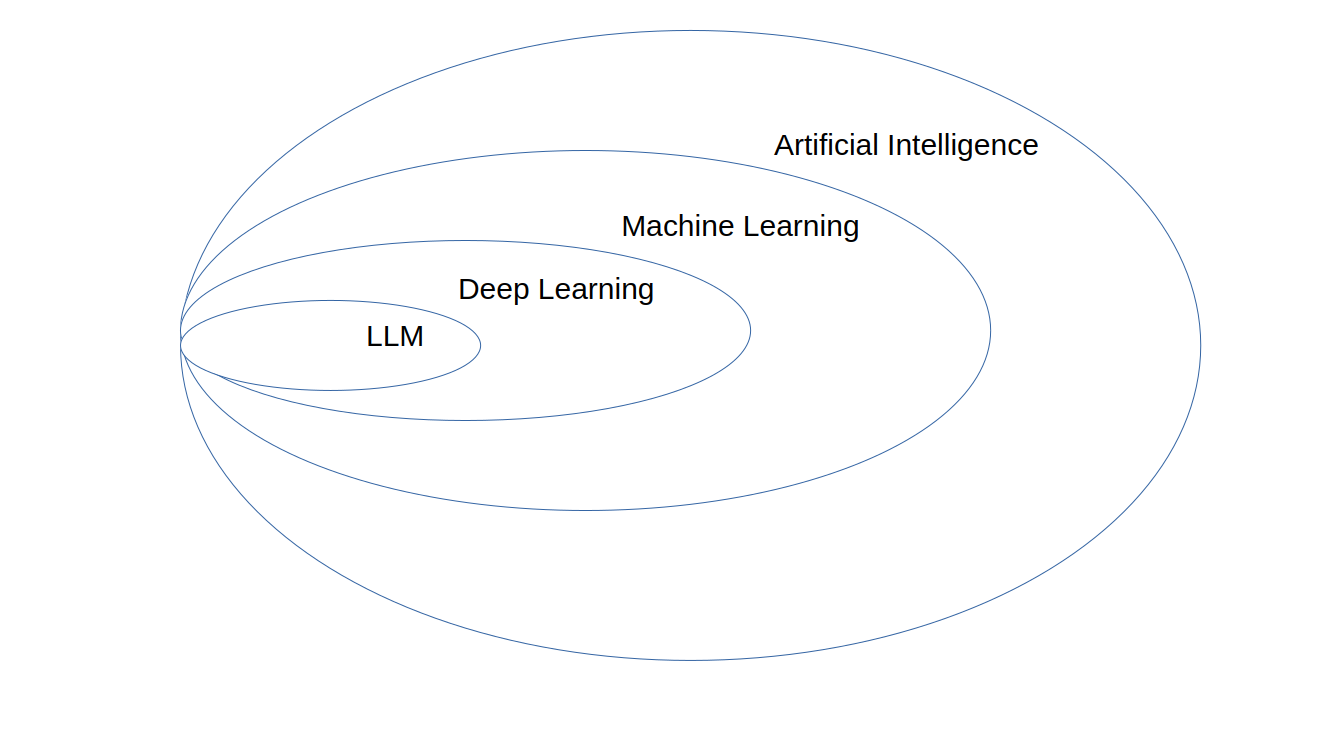
\includegraphics[keepaspectratio]{../figures/broader-AI.png}}

\section{Course contents for LLM}\label{course-contents-for-llm}

\pandocbounded{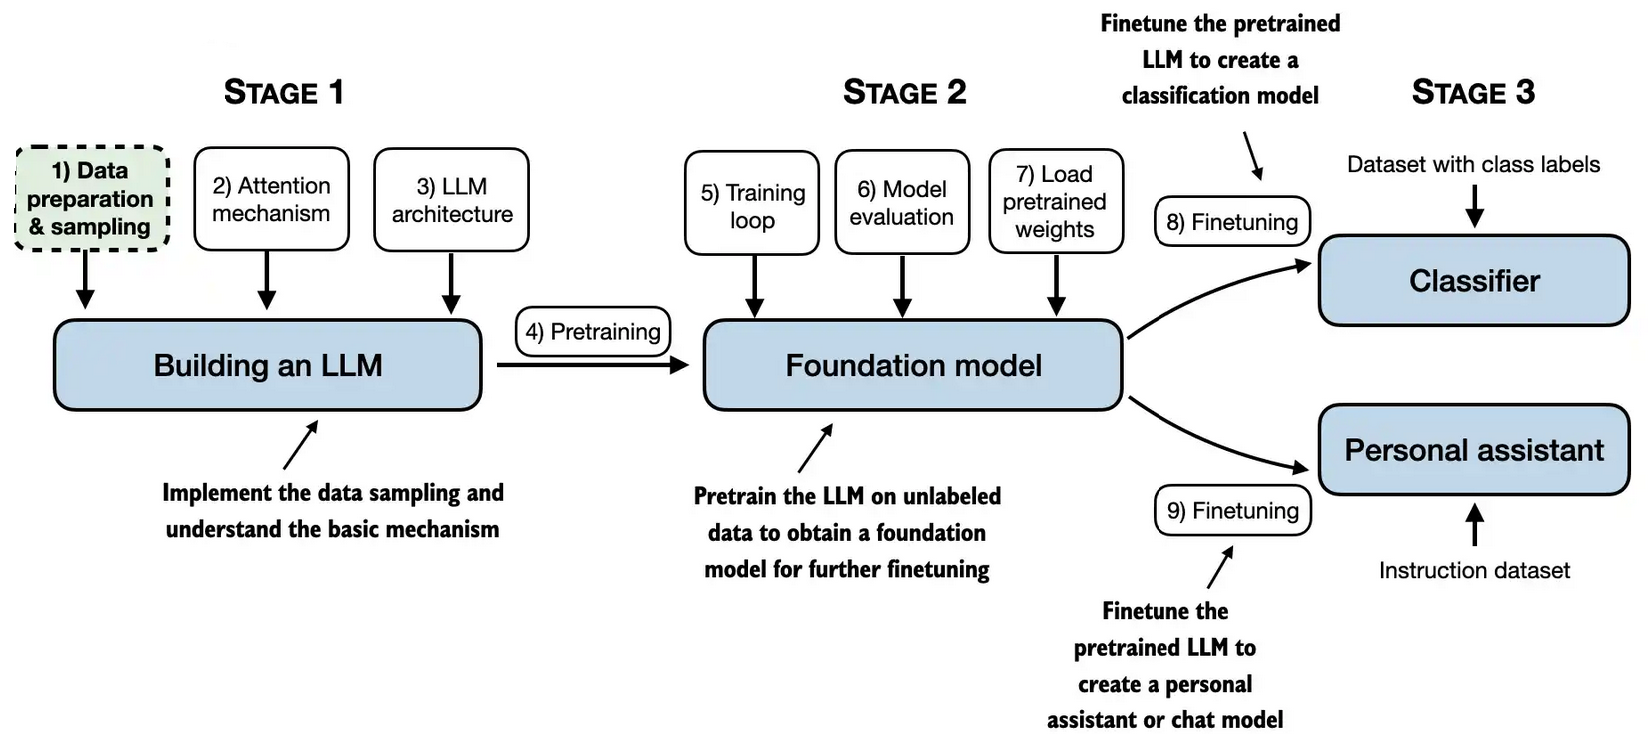
\includegraphics[keepaspectratio]{../images/course-content-LLM.png}}

\subsection{Course book}\label{course-book}

\pandocbounded{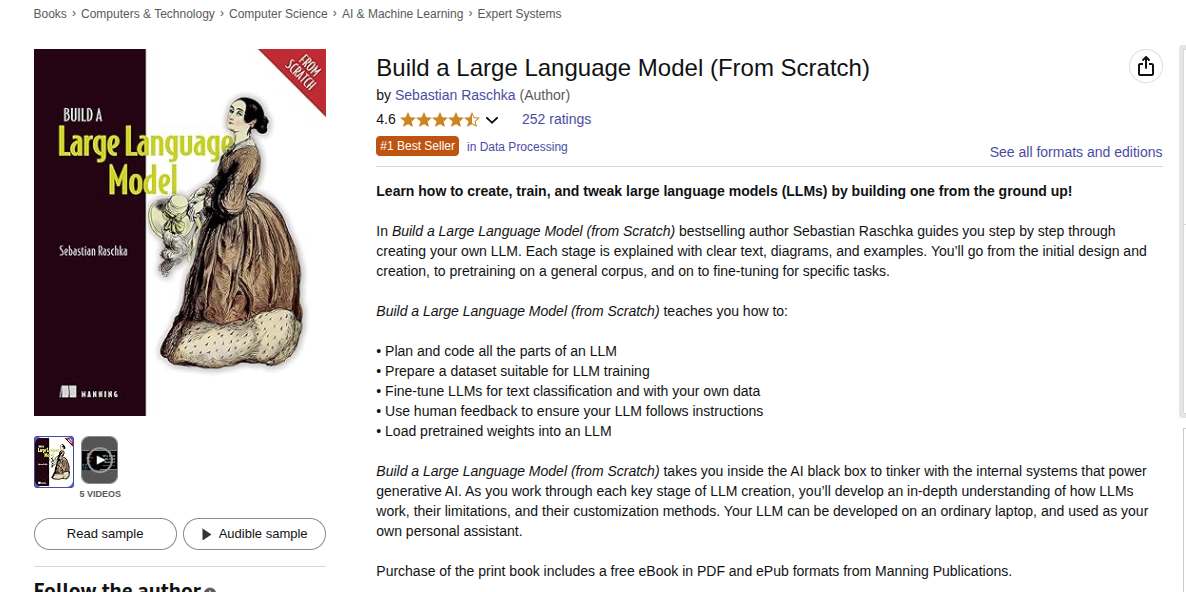
\includegraphics[keepaspectratio]{../images/book-build-a-large-language-model-from-scratch.png}}

\section{How Large Language Models (LLMs)
work}\label{how-large-language-models-llms-work}

LLMs are built using supervised learning. They repeatedly predict next
words using previous words.

\textbf{My favorite food is a Döner with spicy souse}

\begin{longtable}[]{@{}ll@{}}
\toprule\noalign{}
Input A & Output \\
\midrule\noalign{}
\endhead
\bottomrule\noalign{}
\endlastfoot
My & favorite \\
My favorite & food \\
My favorite food & is \\
My favorite food is & a \\
My favorite food is a & Döner \\
My favorite food is a Döner & with \\
My favorite food is a Döner with & spicy \\
My favorite food is a Döner with spicy & souse \\
\end{longtable}

\subsection{How Large Language Models (LLMs) work
2}\label{how-large-language-models-llms-work-2}

\pandocbounded{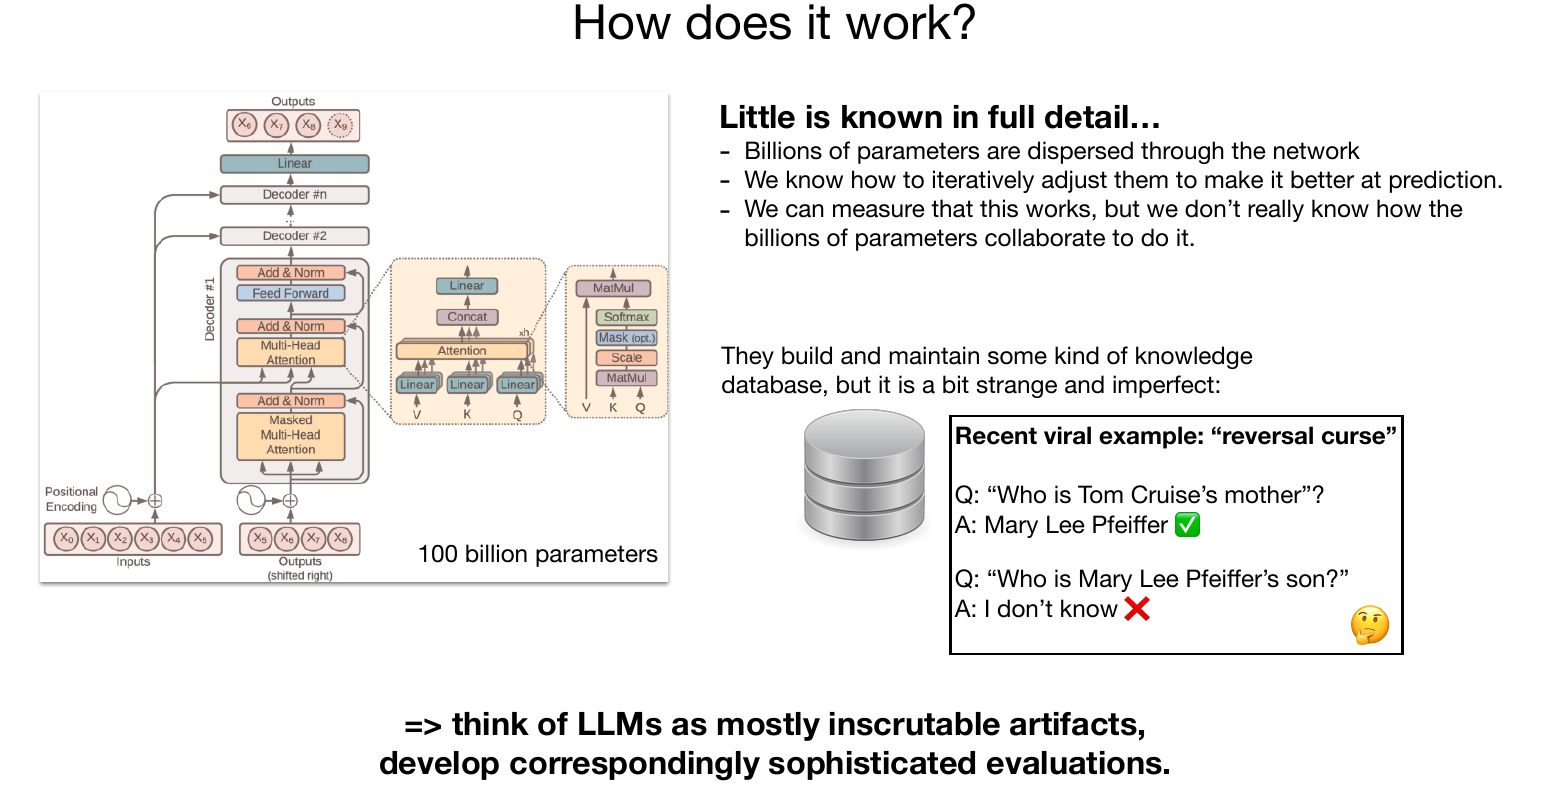
\includegraphics[keepaspectratio]{../images/LLM-how-does-it-work.png}}

\href{https://www.youtube.com/watch?v=7xTGNNLPyMI}{source Andrej
Karpathy: Deep Dive into LLMs like ChatGPT}

\subsection{Stochastic Parrots}\label{stochastic-parrots}

\begin{itemize}
\tightlist
\item
  the term stochastic parrot is a disparaging metaphor, introduced by
  Emily M. Bender and colleagues in a 2021 paper, that frames large
  language models as systems that statistically mimic text without real
  understanding.
\end{itemize}

\pandocbounded{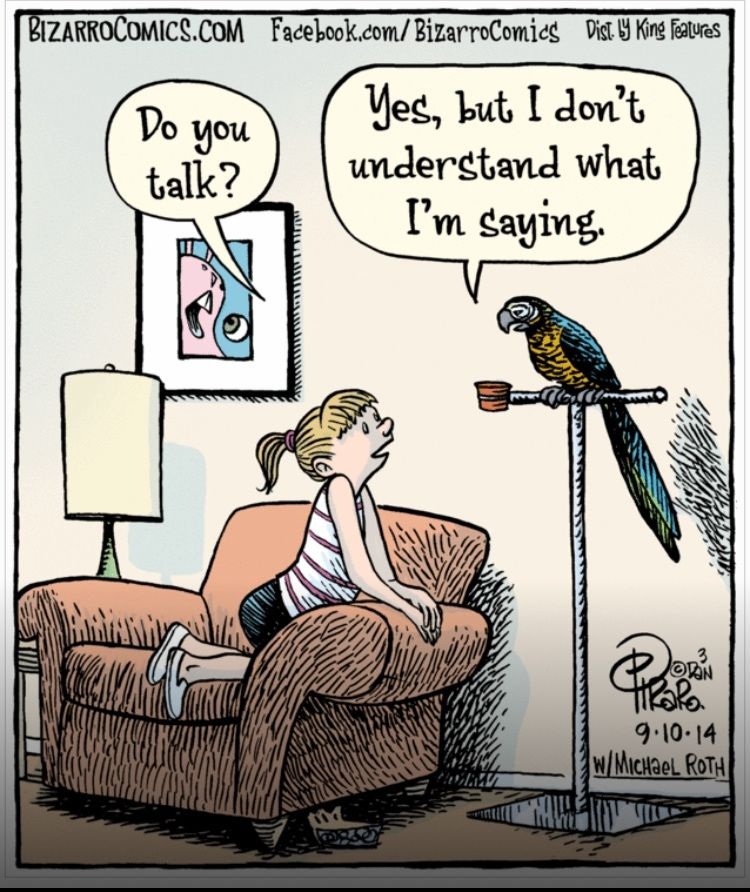
\includegraphics[keepaspectratio]{../images/Stochastic-Parrots.jpeg}}

\subsection{Neural networks}\label{neural-networks}

\pandocbounded{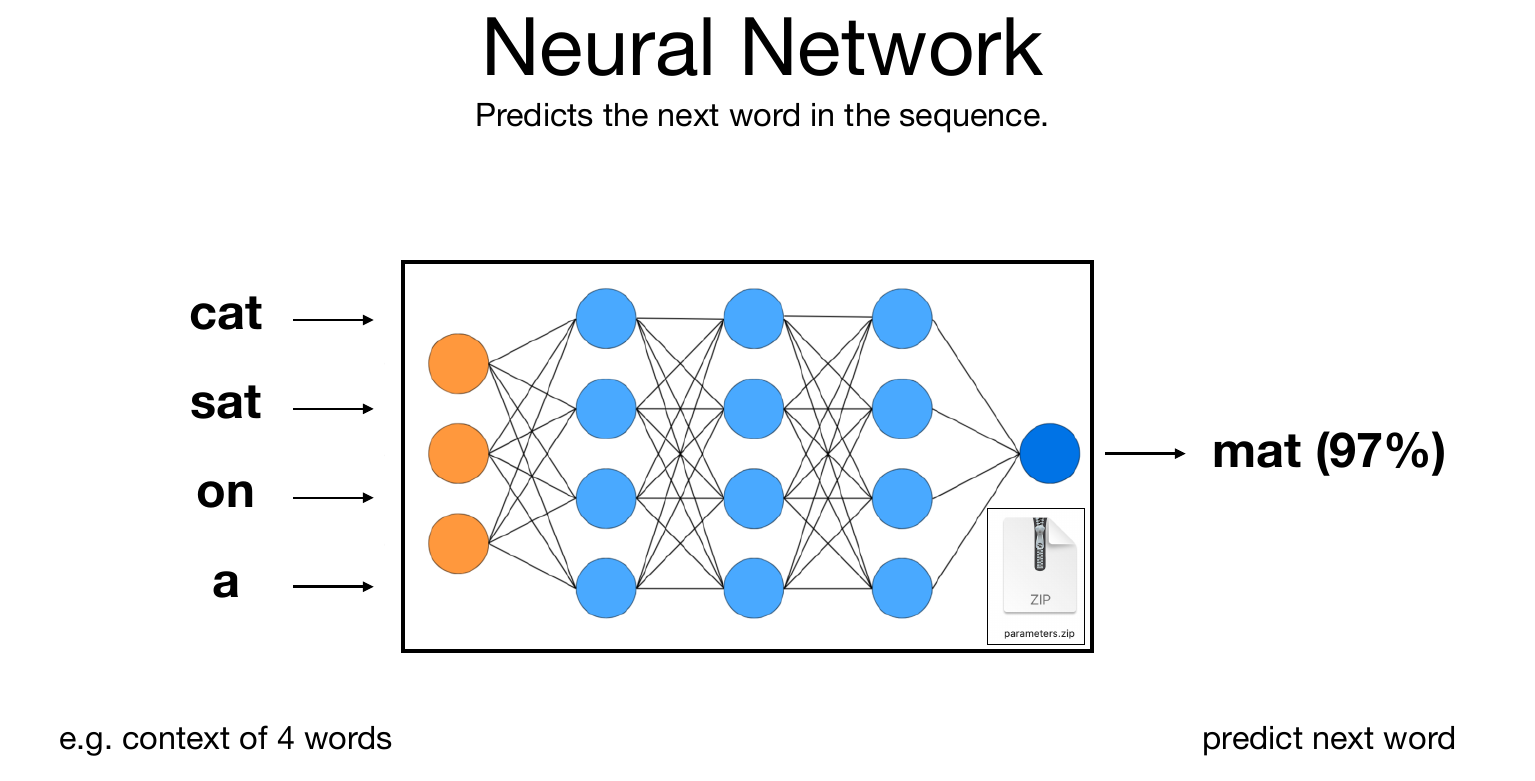
\includegraphics[keepaspectratio]{../images/neural-network.png}}

\href{https://www.youtube.com/watch?v=zjkBMFhNj_g}{Source Andrej
Karpathy: 1hr Talk Intro to Large Language Models}

\subsection{Single Neuron}\label{single-neuron}

\pandocbounded{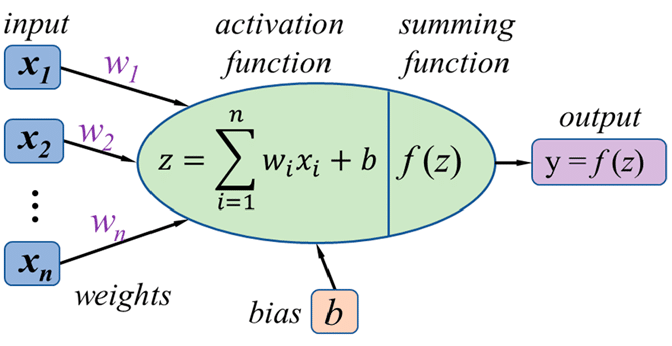
\includegraphics[keepaspectratio]{../images/neuron-bias.png}}

\href{https://discuss.pytorch.org/t/how-to-separate-each-neurons-weights-and-bias-values-for-convolution-and-fc-layers/136800/2}{source}

\subsection{Different activation
functions}\label{different-activation-functions}

\begin{itemize}
\tightlist
\item
  Sigmoid, widely used in old NN papers, is not here
\item
  GELU, GPT activation function, is not here also
\item
  More than 20 activation functions exist
\item
  More activation functions are proposed continuously
\end{itemize}

\pandocbounded{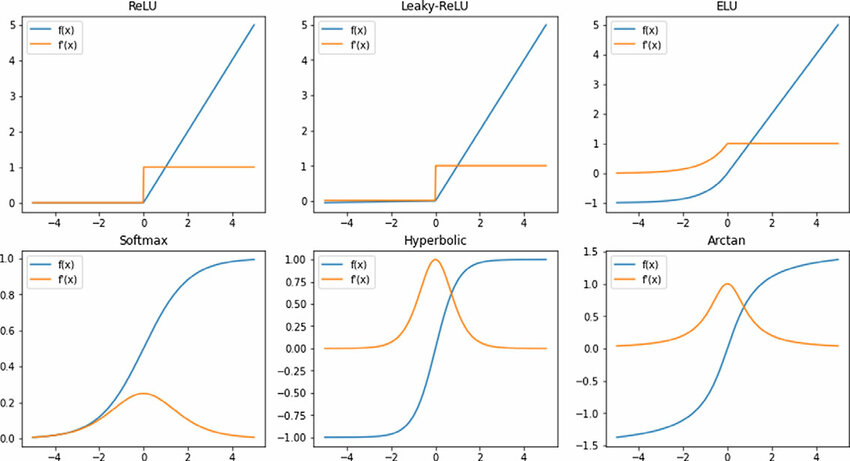
\includegraphics[keepaspectratio]{../images/Commonly-used-activation-functions-fx-and-their-derivatives.jpg}}

\href{https://www.cambridge.org/core/journals/knowledge-engineering-review/article/scalable-speciesbased-genetic-algorithm-for-reinforcement-learning-problems/F81D312989BA030713E7CC2E87D20AC7\#figures-tab}{source:
A scalable species-based genetic algorithm for reinforcement learning
problems}

\subsection{Neural networks internals}\label{neural-networks-internals}

\pandocbounded{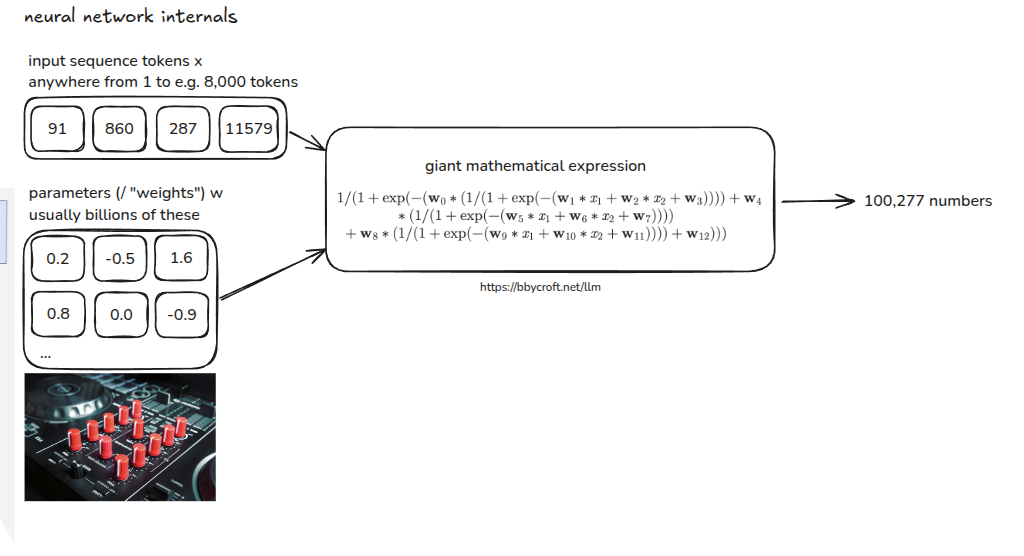
\includegraphics[keepaspectratio]{../images/neural-network-internals.png}}

\href{https://www.youtube.com/watch?v=7xTGNNLPyMI}{source Andrej
Karpathy: Deep Dive into LLMs like ChatGPT}

\subsection{Sources}\label{sources}

\subsubsection{Andrej Karpathy}\label{andrej-karpathy}

\begin{itemize}
\tightlist
\item
  \href{https://www.youtube.com/watch?v=zjkBMFhNj_g}{Video: 1hr Talk
  Intro to Large Language Models}
\item
  \href{https://drive.google.com/file/d/1pxx_ZI7O-Nwl7ZLNk5hI3WzAsTLwvNU7/view}{slides:
  1hr Talk Intro to Large Language Models}
\item
  \href{https://www.youtube.com/watch?v=7xTGNNLPyMI}{Video: Deep Dive
  into LLMs like ChatGPT}
\item
  \href{todo\%20add}{Slides:}
\end{itemize}

-\href{https://www.youtube.com/watch?v=7xTGNNLPyMI}{source Andrej
Karpathy: Deep Dive into LLMs like ChatGPT}




\end{document}
